\chapter{Introduction}
\label{chapter:introduction}

\section{About This Research}
\label{section:intro about}

The world is facing an environmental crisis and all organisations and individuals need to play their part in addressing climate change. We have already overstepped key planetary boundaries \citep{Steffen2015} and are continuing to cause irreversible problems. The longer we delay in reducing carbon emissions to zero, the greater will be the cumulative impact on the whole world \citep{Pierrehumbert2019}.

This research concentrates on the environmental impact of Information and Communication Technology (\gls{ICT}). ICT is important because it participates in both sides of the \gls{sustainability ledger} \todo{elaborate on this `ledger'}. Computer systems can aid in any of the \gls{un goals}, for example by reducing travel through virtual meetings, calculating fuel-efficient delivery routes, or controlling agricultural machinery for greater crop yields. However, the manufacturing, operation, and disposal of such systems has a large environmental cost. Estimates show the ICT sector contributing between 4-5\% of the total greenhouse gas emissions world-wide \citep{Belkhir2018}. To put this in perspective, this proportion is roughly twice the emissions due to air travel. \citet{Penzenstadler2013} drew the distinction between the use of computer technology \emph{for} sustainability and the sustainability \emph{of} that technology. \citep{Becker2023} takes this further and suggests that computing is `insolvent' and may never be able to pay back its environmental and social costs.

This research concentrates on sustainability \emph{of} rather than \emph{for}.

Computer technology is important because it is \emph{changeable}. Unlike, say, a steam engine or door hinge, which once constructed can only work in one way, computer systems can be reprogrammed to perform similar or different tasks in different ways. Although it is mainly the physical aspect of computer systems which requires resources to construct or dispose of and which consumes energy to operate, that hardware is controlled by software which has the potential to increase or reduce the amount of resources and energy required. The potential environmental impact of changes to software is twofold:

\begin{enumerate}
\item software changes can affect the operational energy requirements of a particular hardware system.
\item software changes can also increase or reduce the amount of ICT hardware required to address a particular need.
\end{enumerate}

Real computer systems are often large (in the sense of many parts rather than physical size), complex, and very difficult for any one person to fully understand \todo{citation}. I have spent over 30 years working in software development and have observed first hand how difficult it can be to determine whether any particular choice or change may result in a positive or negative contribution to the end result. The aim of this research is to explore some potential contributions to the huge problem of making ICT systems more sustainable.

\todo{note on software size?}

\section{Summary of Contributions To Knowledge}
\label{section:contrib summary}

This research has generated several contributions to knowledge, which are listed in \autoref{table:contributions}. Individual contributions are discussed in more detail in \autoref{section:contributions}.

\begin{table}[htbp]
\centering
\begin{tabular}{rll}
\makecell[tl]{1} & \makecell[tl]{A Novel Self-Contained Apparatus for Comparing Software \\ Performance and Energy Consumption \emph{(\autoref{contrib:apparatus})}} \\
\makecell[tl]{2} & \makecell[tl]{Energy Use and Performance Comparisons for a Cohort of \\ Web Server Implementations \emph{(\autoref{contrib:servers})}} \\
\makecell[tl]{3} & \makecell[tl]{The Relative Energy Usage of WordPress Compared to \\ Static Websites \emph{(\autoref{contrib:wordpress})}} \\
\makecell[tl]{4} & \makecell[tl]{A Novel Extendable Java Framework for Template Engine \\ Comparison \emph{(\autoref{contrib:framework})}} \\
\makecell[tl]{5} & \makecell[tl]{A Novel Intermediate Language and Generation Tools for \\ Templated Systems \emph{(\autoref{contrib:gilt})}} \\
\makecell[tl]{6} & \makecell[tl]{Energy Use and Performance Comparisons for a Cohort of \\ Template Engine Implementations \emph{(\autoref{contrib:engines})}} \\
\makecell[tl]{7} & \makecell[tl]{A Challenge to the Notion of Execution Speed as a Proxy for \\ Software Energy Usage \emph{(\autoref{contrib:speed as proxy})}} \\
\makecell[tl]{8} & \makecell[tl]{A Challenge to the Notion of Task Complexity as a Proxy for \\ Software Energy Usage \emph{(\autoref{contrib:complexity as proxy})}} \\
\makecell[tl]{9} & \makecell[tl]{The Efficacy of Component Substitution as a Strategy to \\ Improve Software Sustainability \emph{(\autoref{contrib:efficacy})}} \\
\end{tabular}
\caption{Contributions to Knowledge\label{table:contributions}}
\end{table}


\section{Mapping to UN Sustainability Goals}
\label{section:un goals}

The United Nations (UN) has set out seventeen `Sustainable Development Goals'  [\autoref{17-goals-image}]. This research contributes to Goal 13 (\emph{Climate Action}) by addressing the climate impact of Goals 9 (\emph{Industry, Innovation, and Infrastructure}) and 12 (\emph{Responsible Consumption and Production}).

\todo{elaborate} 

\begin{figure}[ht!]
\centering
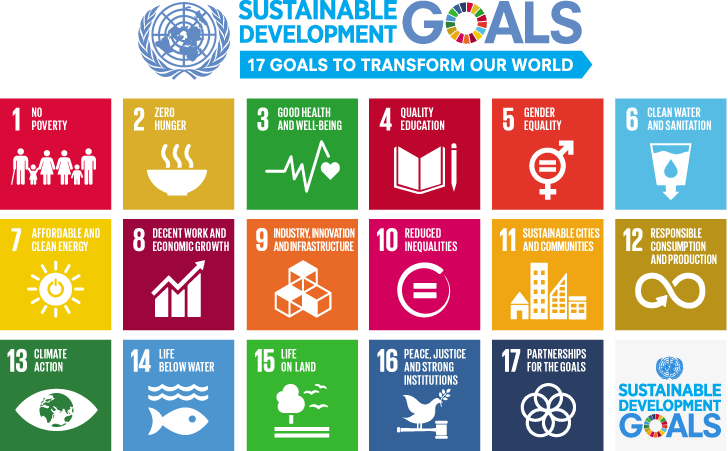
\includegraphics[width=\textwidth]{Figures/17goals.png}
\caption{\label{17-goals-image}The 17 \gls{un goals} \citep{UnitedNations2015}}
\end{figure}

\section{Thesis Structure}
\label{section:thesis structure}

The main content of this thesis comprises a series of studies exploring different aspects of the bigger picture, brought together at the end for combined reflection and conclusions.

\paragraph{\autoref{chapter:context}} introduces the context of the research including the scale of the sustainability issues of ICT systems, a brief introduction to the history of computers and software and what is currently being done by the computer industry to address sustainability, and an exploration of how software is made.

\paragraph{\autoref{chapter:questions}} clarifies some key terminology and explores literature and related research before identifying a research gap and defining some research objectives.

\paragraph{\autoref{chapter:performance}} explores the differences in performance between a representative cohort of software components under differing usage scenarios then designs, constructs, and evaluates a framework to simplify component substitution.

\paragraph{\autoref{chapter:testrig}} designs, constructs, and evaluates a low-cost, self-contained apparatus for the comparison of software energy usage. The apparatus is used to compare performance and energy usage of a range of web server applications, both when serving `static' websites and when using the popular \emph{WordPress} content management application.

\paragraph{\autoref{chapter:intermediate}} explores the differences between the template languages used to represent web page templates and constructs an intermediate language and a software tool to generate templates for a range of different template engines from a single source template.

\paragraph{\autoref{chapter:comp energy}} explores the use of the comparison apparatus from \autoref{chapter:testrig}, the substitution framework developed in \autoref{chapter:performance}, and the template format and tools from \autoref{chapter:intermediate} to investigate and compare the performance and energy use of template engine components under different scenarios.

\paragraph{\autoref{chapter:conclusions}} reflects and summarises the outcomes of the research from previous chapters.